\section{Tests des modèles par variation de paramètres}
Dans le cours de Neural Network and Learning nous avons vue qu’il était important de faire varier les paramètres dans le but de faire augmenter l’accuracy et diminué le taux d’erreur.\\
Pour chaque méthodes le taux d’erreur a était calculé de manière identique. Nous avons repris les résumés de la base de données initial, les avons classés grâce à la méthode testée puis nous en avons fait un pourcentage d’erreur.\\
Dans les sections \ref{variation_SVM} et \ref{variation_LogisticRegression}  nous avons fait varier les paramètres test\_size et train\_size de 0.1 à 0.9 avec la contrainte que la somme de ces dernières doit être inférieur à 1.

\subsection{SVM} \label{variation_SVM}
Pour illustrer la variation de l’accuracy et du taux d’erreur nous avons réalisé des graphiques. Pour des raisons de lisibilité nous avons fait plusieurs graphiques, vous pouvez donc voire ici le graphique comportent le meilleur résultat que nous ayons obtenue pour SVM, 58\% d’accuracy pour 43\% d’erreur, pour test\_size = 0.1 et train\_size = 0.5.
\begin{center}
    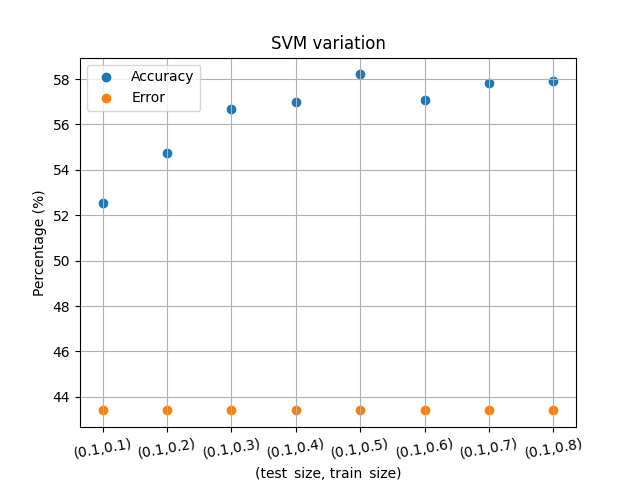
\includegraphics[scale=1]{graphs/svm-variation-0.png}
    \captionof{figure}{SVM variation}
\end{center}

\newpage

\subsection{LogisticRegression}
Vous pouvez également voire ici le graphique comportent le meilleur résultat que nous ayons obtenue pour LogisticRegression, 58\% d’accuracy pour 42\% d’erreur, pour test\_size = 0.2 et train\_size = 0.7.
\label{variation_LogisticRegression}

\begin{center}
    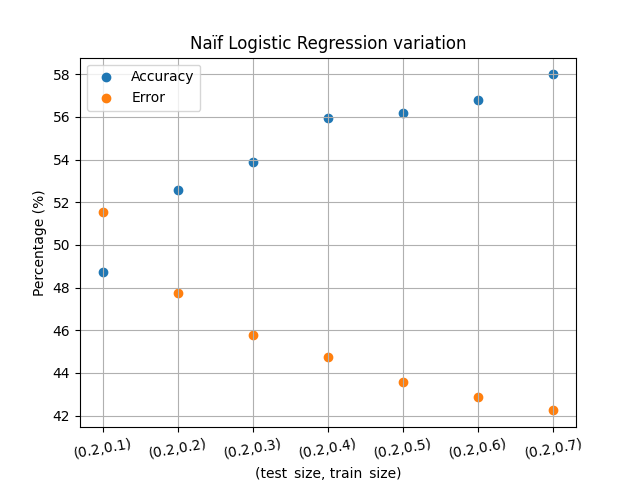
\includegraphics[scale=1]{graphs/variation-error_accuracy-1.png}
    \captionof{figure}{LogisticRegression variation}
\end{center}

\newpage
\subsection{MLPClassifier}
MLP étant un modèle de réseau de neurones nous avons fait varier le nombre de couche ainsi que le nombre de neurones par couche.\\
Comme pour les graphiques précédents on voit uniquement celui comportant le meilleur résultat, 55\% d’accuracy pour 46\% d’erreur, pour 1 couche composée de 46 neurones.

Nous avons décidé de prendre test\_size=0.2 et train\_size=0.7 comme LogisticRegression car nous n'avons pas eu le temps de faire les tests pour chaque paramètre.

\label{variation_LogisticRegression}

\begin{center}
    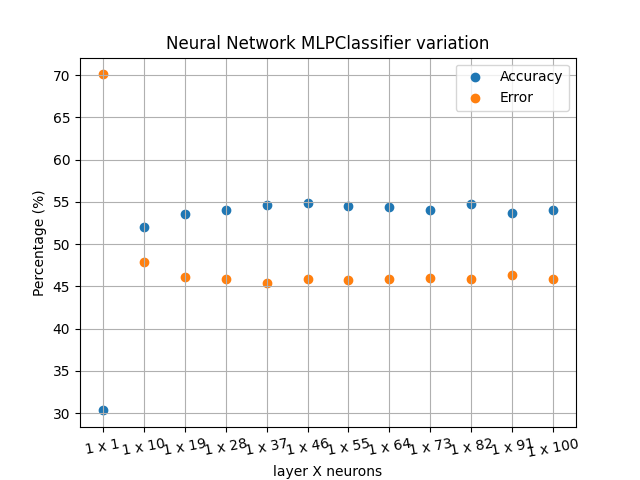
\includegraphics[scale=1]{graphs/neural_network_variation-error_accuracy-0.png}
    \captionof{figure}{MLPClassifier variation}
\end{center}